\documentclass{article}
\usepackage{tikz}
\usetikzlibrary{arrows.meta, positioning, quotes}

\begin{document}

\begin{figure}[h]
    \centering
    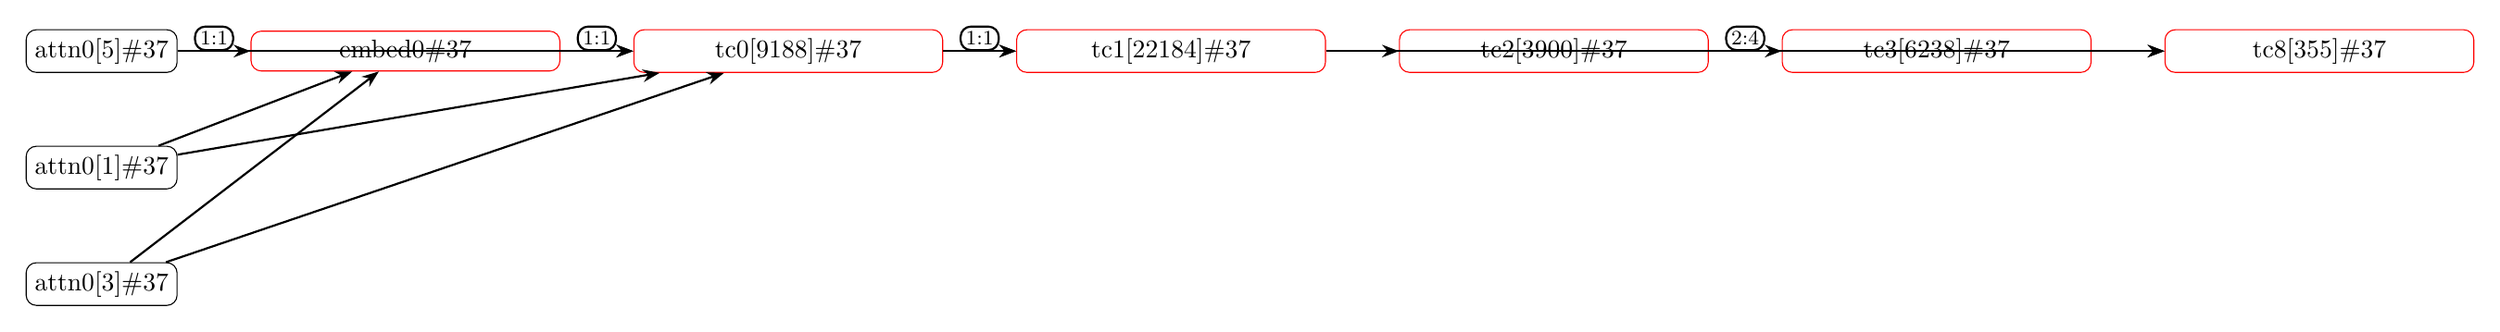
\begin{tikzpicture}[node distance=1cm, auto,
        every node/.style={draw, rounded corners},
        every edge/.style={draw, -Stealth, thick},
        every edge quotes/.style={auto, font=\footnotesize, inner sep=2pt}
    ]
    
    % Nodes
    \node (att0) {attn0[5]\#37};
    \node [below=of att0] (att1) {attn0[1]\#37};
    \node [below=of att1] (att2) {attn0[3]\#37};
    \node [right=of att0, text width=4cm, align=center, draw=red, rounded corners] (embed) {embed0\#37};
    \node [right=of embed, text width=4cm, align=center, draw=red, rounded corners] (tc0) {tc0[9188]\#37};
    \node [right=of tc0, text width=4cm, align=center, draw=red, rounded corners] (tc1) {tc1[22184]\#37};
    \node [right=of tc1, text width=4cm, align=center, draw=red, rounded corners] (tc2) {tc2[3900]\#37};
    \node [right=of tc2, text width=4cm, align=center, draw=red, rounded corners] (tc3) {tc3[6238]\#37};
    \node [right=of tc3, text width=4cm, align=center, draw=red, rounded corners] (tc8) {tc8[355]\#37};

    % Edges
    \path
        (att0) edge ["1:1"] (embed)
        (embed) edge ["1:1"] (tc0)
        (tc0) edge ["1:1"] (tc1)
        (tc1) edge ["2:4"] (tc8)
        (att1) edge (embed)
        (att2) edge (embed)
        (att0) edge (tc0)
        (att1) edge (tc0)
        (att2) edge (tc0)
        (tc0) edge (tc1)
        (tc1) edge (tc2)
        (tc2) edge (tc3)
        (tc3) edge (tc8);
    \end{tikzpicture}
    \caption{An example of a computational graph produced using the method in \S\ref{sec:subgraphs} characterizing how our unknown feature is computed on an unseen input. A single path is highlighted in red and annotated with component-by-component attributions.}
    \label{fig:computational_graph}
\end{figure}

\end{document}